\documentclass[
11pt,%
tightenlines,%
twoside,%
onecolumn,%
nofloats,%
nobibnotes,%
nofootinbib,%
superscriptaddress,%
noshowpacs,%
centertags]%
{revtex4}
\usepackage{ljm}
\usepackage{listings}
\usepackage{amsmath}

\lstset{
language=C++,
basewidth=0.5em,
xleftmargin=45pt,
xrightmargin=45pt,
basicstyle=\small\ttfamily,
keywordstyle=\bfseries\underbar,
numbers=left,
numberstyle=\tiny,
stepnumber=1,
numbersep=10pt,
showspaces=false,
showstringspaces=false,
showtabs=false,
frame=trBL,
tabsize=2,
captionpos=t,
breaklines=true,
breakatwhitespace=false,
escapeinside={\%*}{*)}
}

\begin{document}

\titlerunning{solving nonlinear equations}
\authorrunning{Bagrov, Rybakov}

\title{Selection of a method for solving nonlinear equations in shallow-water icing model implementation}

\author{\firstname{A.~D.}~\surname{Bagrov}}
\email[E-mail: ]{andrey.bagrov@yandex.ru}
\affiliation{Joint Supercomputer Center of the Russian Academy of Sciences -- branch of Scientific Research Institute of System Analysis of the Russian Academy of Sciences, Leninsky prospect 32a, Moscow, 119334, Russia}

\author{\firstname{A.~A.}~\surname{Rybakov}}
\email[E-mail: ]{rybakov.aax@gmail.com}
\affiliation{Joint Supercomputer Center of the Russian Academy of Sciences -- branch of Scientific Research Institute of System Analysis of the Russian Academy of Sciences, Leninsky prospect 32a, Moscow, 119334, Russia}

\firstcollaboration{(Submitted by TODO)} % Add if you know submitter.
%\lastcollaboration{ }

\received{TODO}

\begin{abstract}
Моделирование ледяных наростов на профилях летательных аппаратов в процессе их полета в среде, содержащей переохлажденные капли воды, является крайней важной задачей для безопасности полетов, так как образуемые ледяные наросты существенным образом влияют на летные характеристики.
В одной из моделей решения поставленной задачи -- shallow-water icing model (SWIM) -- центральную роль в численном моделировании занимает задача решения нелинейных уравнений с одной переменной.
Так как данная задача занимает подавляюще большую часть всех расчетов, то вопрос выбора оптимального метода решения нелинейных уравнений и оптимизации данных методов встает особенно остро.
В данной статье описан анализ использования различных методов решения нелинейных уравнений в реализации решателя SWIM с учетом особенностей решаемых уравнений, что привело к существенному ускорению расчетных кодов при выполнении вычислений на суперкомпьютерах МСЦ РАН.
\end{abstract}

\subclass{65H05, 65Y20} % Enter 2010 Mathematics Subject Classification.

\keywords{nonlinear equations, shallow-water icing model, bisections method, Newton's method, Brent's method}

\maketitle

\section{Introduction}

В настоящее время известно множество расчетных кодов, использующихся для численного моделирования обледенения поверхности обтекаемого тела.
Одними из наиболее популярных пакетов для решения данной задачи являются Lewice \cite{Wright} и ONERA.
В данной статье мы не будем касаться особенностей данных расчетных пакетов и различий между ними, а рассмотрим только реализацию решателя SWIM, подробно описанного в \cite{Bourgault}.
При выполнении компьютерного моделировании процесса обледенения поверхности, обтекаемой свободным потоком, в shallow-water icing model выполняется одновременный расчет нарастания льда и течения пленки жидкости по поверхности обтекаемого тела. При этом учитывается выпадение влаги на поверхность тела, испарение влаги или сублимация льда с поверхности тела, течение жидкой пленки по поверхности с частичным ее замерзанием, а также перетекание потоков тепла между телом и поверхностью и между поверхностью и окружающим воздухом.

Численные расчеты выполняются на поверхностной расчетной сетке, состоящей из отдельных ячеек, при этом в каждой ячейке поверхности должен выполняться закон сохранения массы, записываемый в следующем виде:

\begin{equation}
\rho_w \left[ \frac{\partial h_f}{\partial t} + \operatorname{div}(\overline{u} h_f) \right] = U_{\infty} LWC \beta - \dot m_{evap} - \dot m_{ice}
\end{equation}

В данной формуле $\rho_w$ -- плотность воды, $h_f$ -- высота водяной пленки на поверхности, $\overline{u}$ -- скорость течения водяной пленки, $U_{\infty}$ -- скорость набегания свободного потока, $LWC$ -- содержание влаги в набегающем потоке, $\dot m_{evap}$ -- удельная скорость испарения или сублимации с поверхности обтекаемого тела, $\dot m_{ice}$ -- удельная скорость нарастания массы льда.

Кроме того, в каждой ячейке выполняется закон сохранения энергии:

\begin{equation}
\begin{aligned}
& \rho_w \left[ \frac{\partial h_f C_w \tilde{T}}{\partial t} + \operatorname{div}(\overline{u} h_f C_w \tilde{T}) \right] = \left[ C_w \tilde{T}_{d,\infty} + \frac{||\overline{u}_d||^2}{2} \right] \times U_{\infty} LWC \beta
\\
& - \frac{1}{2}(L_{evap} + L_{subl}) \dot m_{evap} + (L_{fusion} - C_{ice} \tilde{T}) \dot m_{ice} + \sigma (T_{\infty}^4 - T^4) + \dot Q_h + \dot Q_{cond}
\end{aligned}
\end{equation}

В данной формуле $C_w$ -- удельная теплоемкость воды, $\tilde{T}$ -- температура ячейки в градусах Цельсия, $\tilde{T}_{d,\infty}$ -- температура выпадающей влаги в градусах Цельсия, $\overline{u}_d$ -- скорость выпадающих на поверхность капель, $L_{evap}$ - скрытая теплота испарения воды, $L_{subl}$ -- скрытая теплота сублимации льда, $L_{fusion}$ -- скрытая теплота плавления льда, $C_{ice}$ -- теплоемкость льда, $\sigma$ -- постоянная Больцмана, $T_{\infty}$ -- температура свободного потока в кельвинах, $T$ - температура ячейки в кельвинах, $\dot Q_h$ -- удельная величина потока тепла, получаемого из воздуха, $\dot Q_{cond}$ -- удельная величина потока тепла, поступающего в ячейку из обтекаемого тела.

Для численного решения приведенной системы уравнений необходимо выполнить ее дискретизацию по времени и пространстрву, как это показано в \cite{Beaugendre}.
После этого получим систему из двух разностных уравнений, в которые входят три неизвестные величины: температура поверхности $\tilde{T}$, высота водяной пленки $h_f$ и высота ледяного нароста $h_{ice}$.  

Также при решении системы уравнений должны выполняться условия совместимости, записываемые в виде

\begin{equation}
\begin{cases}
h_f \ge 0\\
\dot m_{ice} \ge 0\\
h_f \tilde{T} \ge 0\\
\dot m_{ice} \tilde{T} \le 0
\end{cases}
\end{equation}

\begin{figure}[h]
\setcaptionmargin{5mm}
\onelinecaptionstrue
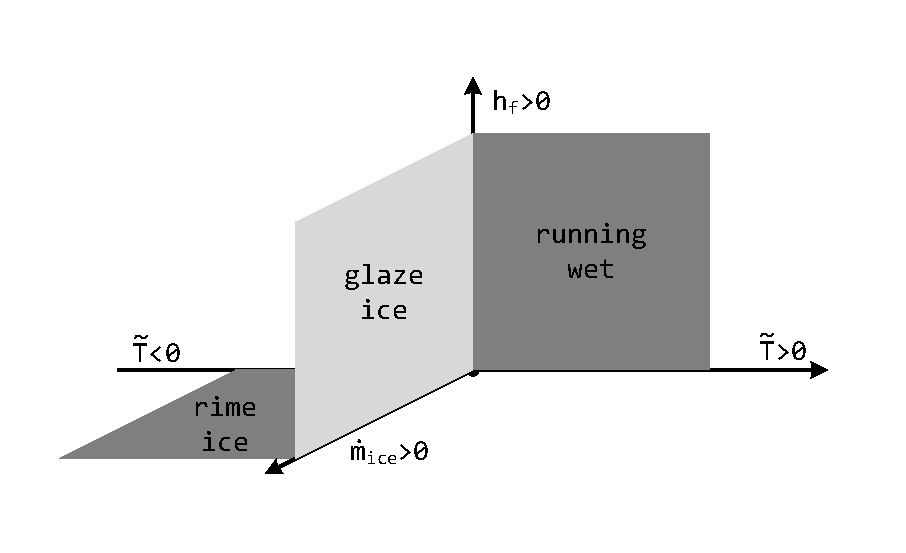
\includegraphics[width=0.7\textwidth]{pics/surface.pdf}
\captionstyle{normal}\caption{Пространство решений системы уравнений массового и теплового баланса ячейки.}\label{fig:surface}
\end{figure}

Несмотря на то, что неизвестных в уравнении больше, чем самих уравнений, система все равно решается, так как данные переменные не являются полностью независимыми.
Решение ищется из условия того, что ячейка может находиться в одном из трех состояний.
Первое состояние -- running wet -- достигается когда в ячейке полностью отсутствует лед и течет жидкая пленка.
В этом случае температура не может быть отрицательной.
Второе состояние -- glaze icing -- если в ячейке одновременно присутствует и лед, и вода.
В этом случае температура равна нулю градусам по Цельсию.
И наконец, в третьем случае при отрицательной температуре в ячейке не может находиться вода и присутствует только лед.
Общее пространство решений показано на Fig.~\ref{fig:surface}.

\section{Features of the equations being solved}

Для состояния ячейки glaze ice система уравнений, состоящая из уравнения массового баланса и уравнения теплового баланса, вырождается в простую систему линейных уравнений с двумя неизвестными (высота водяной пленки и высота ледяного нароста).
Решение такой системы уравнений не представляет сложностей.
Для двух оставшихся состояний ячейки (running wet, rime ice) описанная система уравнений сводится к одному нелинейному уравнению с одной переменной (неизвестной в данном случае является температура ячейки).
При этом в нелинейное уравнение входят такие физические величины как удельная теплоемкость воды, льда и воздуха ($C_w$, $C_{ice}$, $C_a$), скрытое тепло испарения и сублимации ($L_{ev}$, $L_su$), а также динамическая вязкость воды ($\mu_w$).
Данные величины не являются константами, а сами зависят от температуры нелинейным образом.
На Fig.~\ref{fig:ph_graphics_h} показана кусочно-линейная интерполяция данных физических величин, выполненная по их табличным значениям.

\begin{figure}[h]
\setcaptionmargin{5mm}
\onelinecaptionstrue
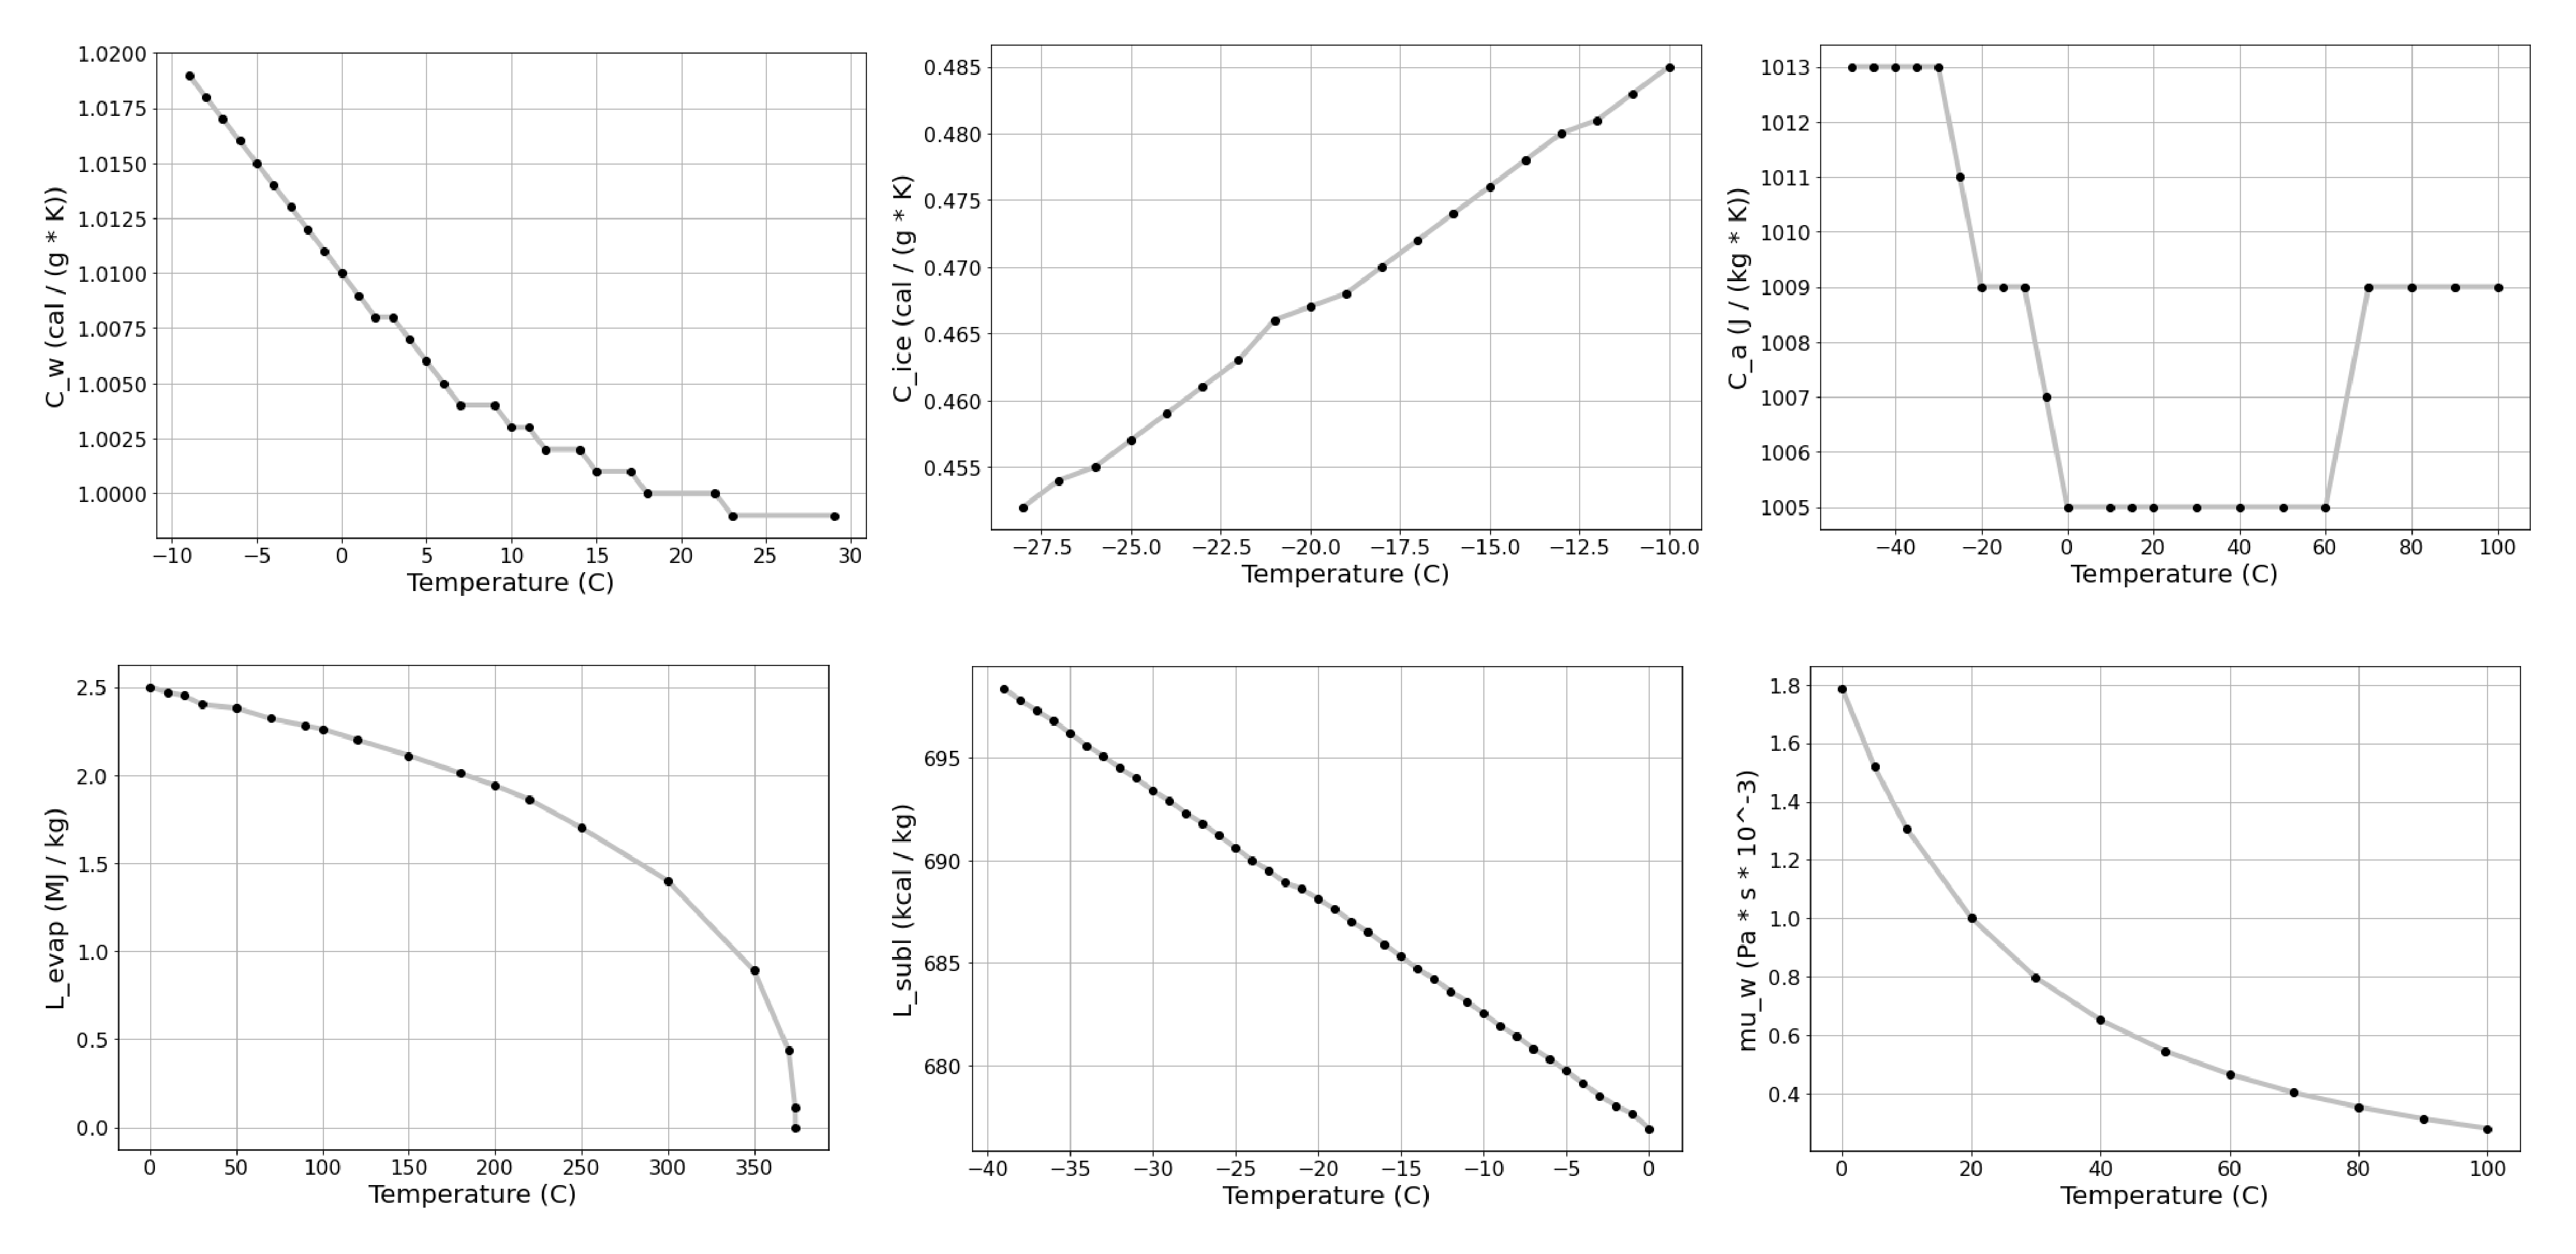
\includegraphics[width=1.0\textwidth]{pics/ph_graphics_h.pdf}
\captionstyle{normal}\caption{Зависимости физических величин от температуры.}\label{fig:ph_graphics_h}
\end{figure}

В процессе выполнения расчетов в масштабах всей поверхности были использованы неструктурированные расчетные сетки с характерным числом ячеек $10^5$, характерное время счета составляет $10^3$ секунд, характерный шаг по времени $10^{-3}$ секунды.
В общем случае на каждом шаге по времени требуется решать нелинейное уравнение от 0 до 2 раз (будем считать, что в среднем 1 раз).
Итого, получаем, что характерное количество запусков решения нелинейного уравнения в процессе запуска типовой расчетной задачи составляет $10^11$ штук.
Такое количество запусков решения нелинейных уравнений является существенных даже при условии распараллеливания вычислений с помощью MPI, OpenMP и применения векторизации программного кода.
Поэтому выбор оптимального метода решения нелинейных уравнений является критически важной задачей для повышения быстродействия программного кода.

При тестировании различных методов решения нелинейных уравнений были собраны профили функций ($f(x)$), для которых требуется найти решение.
Многообразие данных профилей продемонстрировано на Fig.~\ref{fig:dq}.
На этой иллюстрации построены графики семейства функций $f(x)$ для взятых случайным образом ячеек расчетной сетки для случайных моментов времени и для разрешения различных состояний ячеек.

\begin{figure}[h]
\setcaptionmargin{5mm}
\onelinecaptionstrue
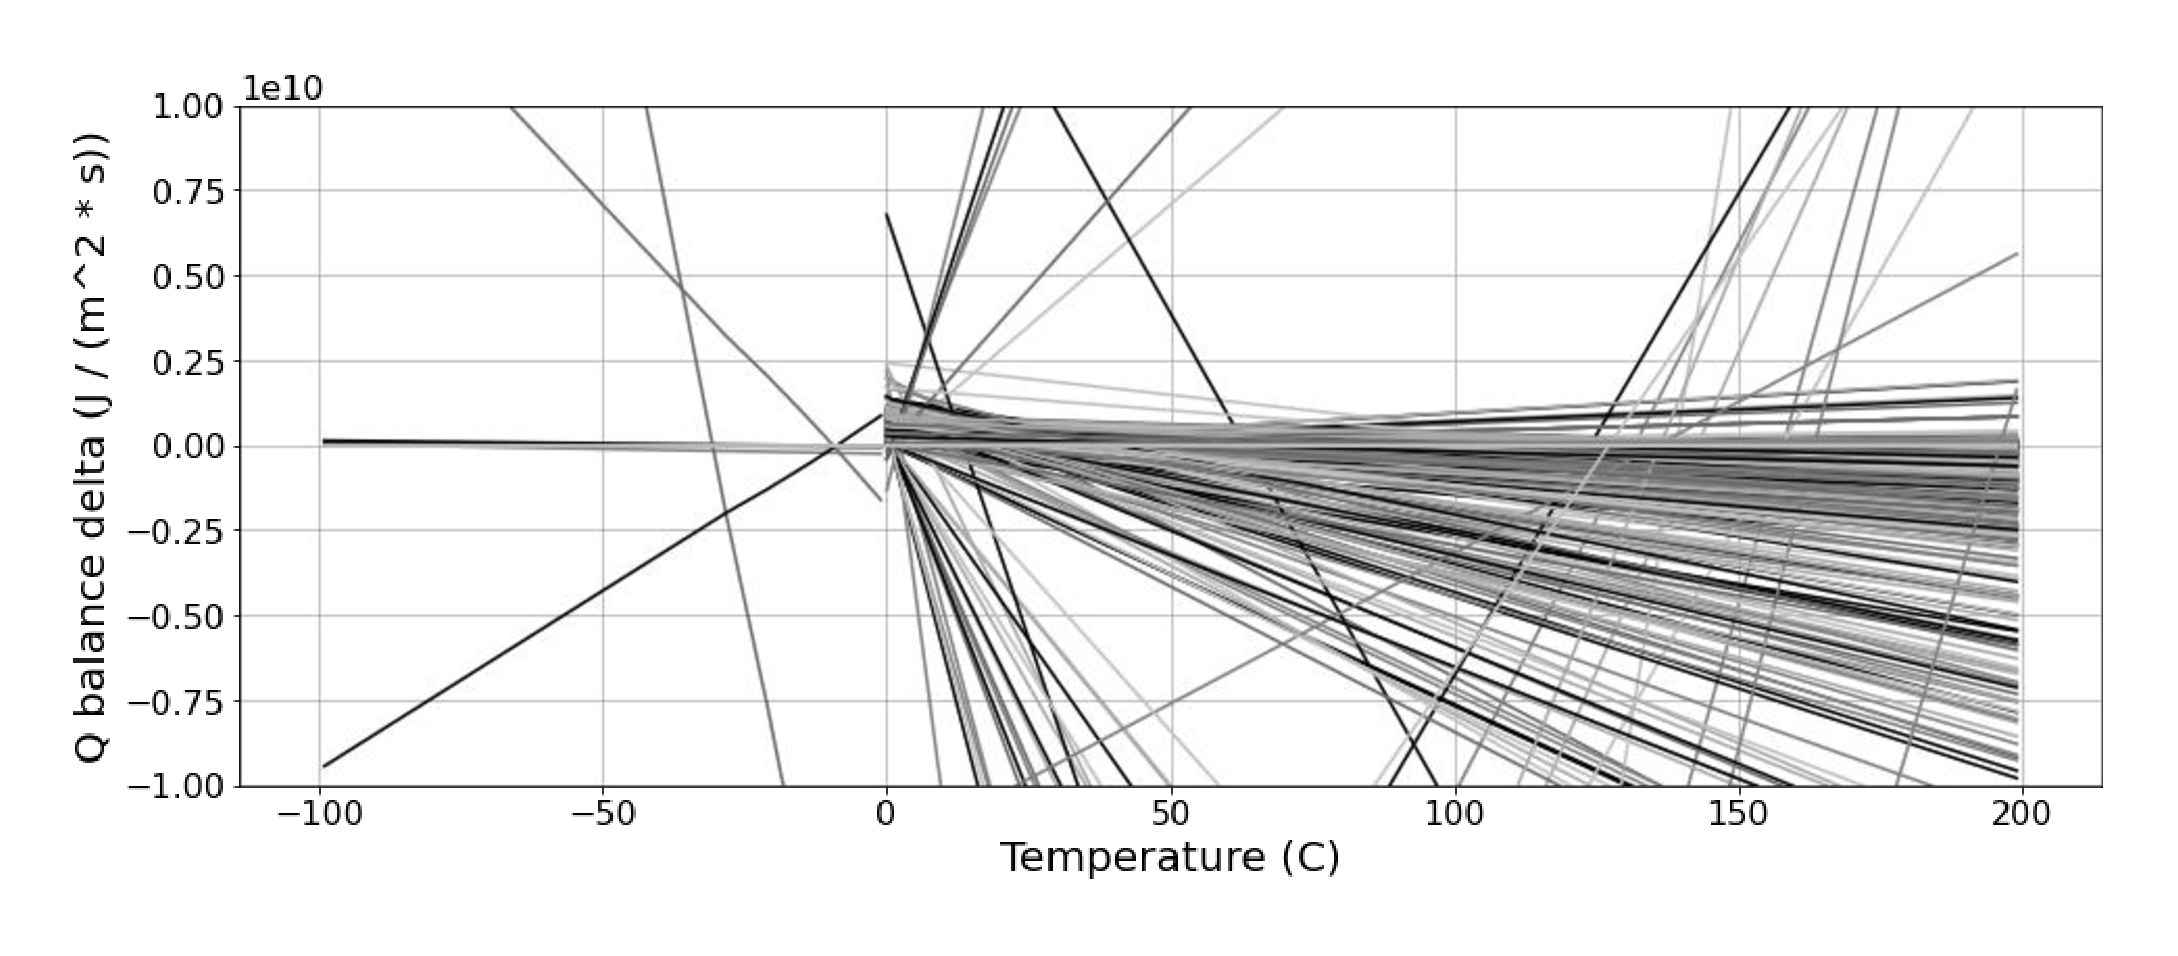
\includegraphics[width=1.0\textwidth]{pics/dq.pdf}
\captionstyle{normal}\caption{Графики функций, представляющих решаемые нелинейные уравнения.}\label{fig:dq}
\end{figure}

Из приведенной иллюстрации может создаться впечатление, что в основном уравнения решались для состояний ячейки running wet (так как область построения графиков $x > 0$ плотно заполнена графиками).
Однако это впечатление ошибочно, просто большинство графиков функций $f(x)$ для состояния ячейки rime ice при данном масштабе сильно прижаты с оси $OX$ и сливаются в один график.
На Fig.~\ref{fig:dq_rime_wet} приведены графики функций для разрешения состояний ячеек rime ice (слева) и running wet (справа) раздельно и в разным масштабах.
На данных графиках можно наблюдать общий вид графиков, представляющих уравнения для разрешения данных двух состояний ячейки.

\begin{figure}[h]
\setcaptionmargin{5mm}
\onelinecaptionstrue
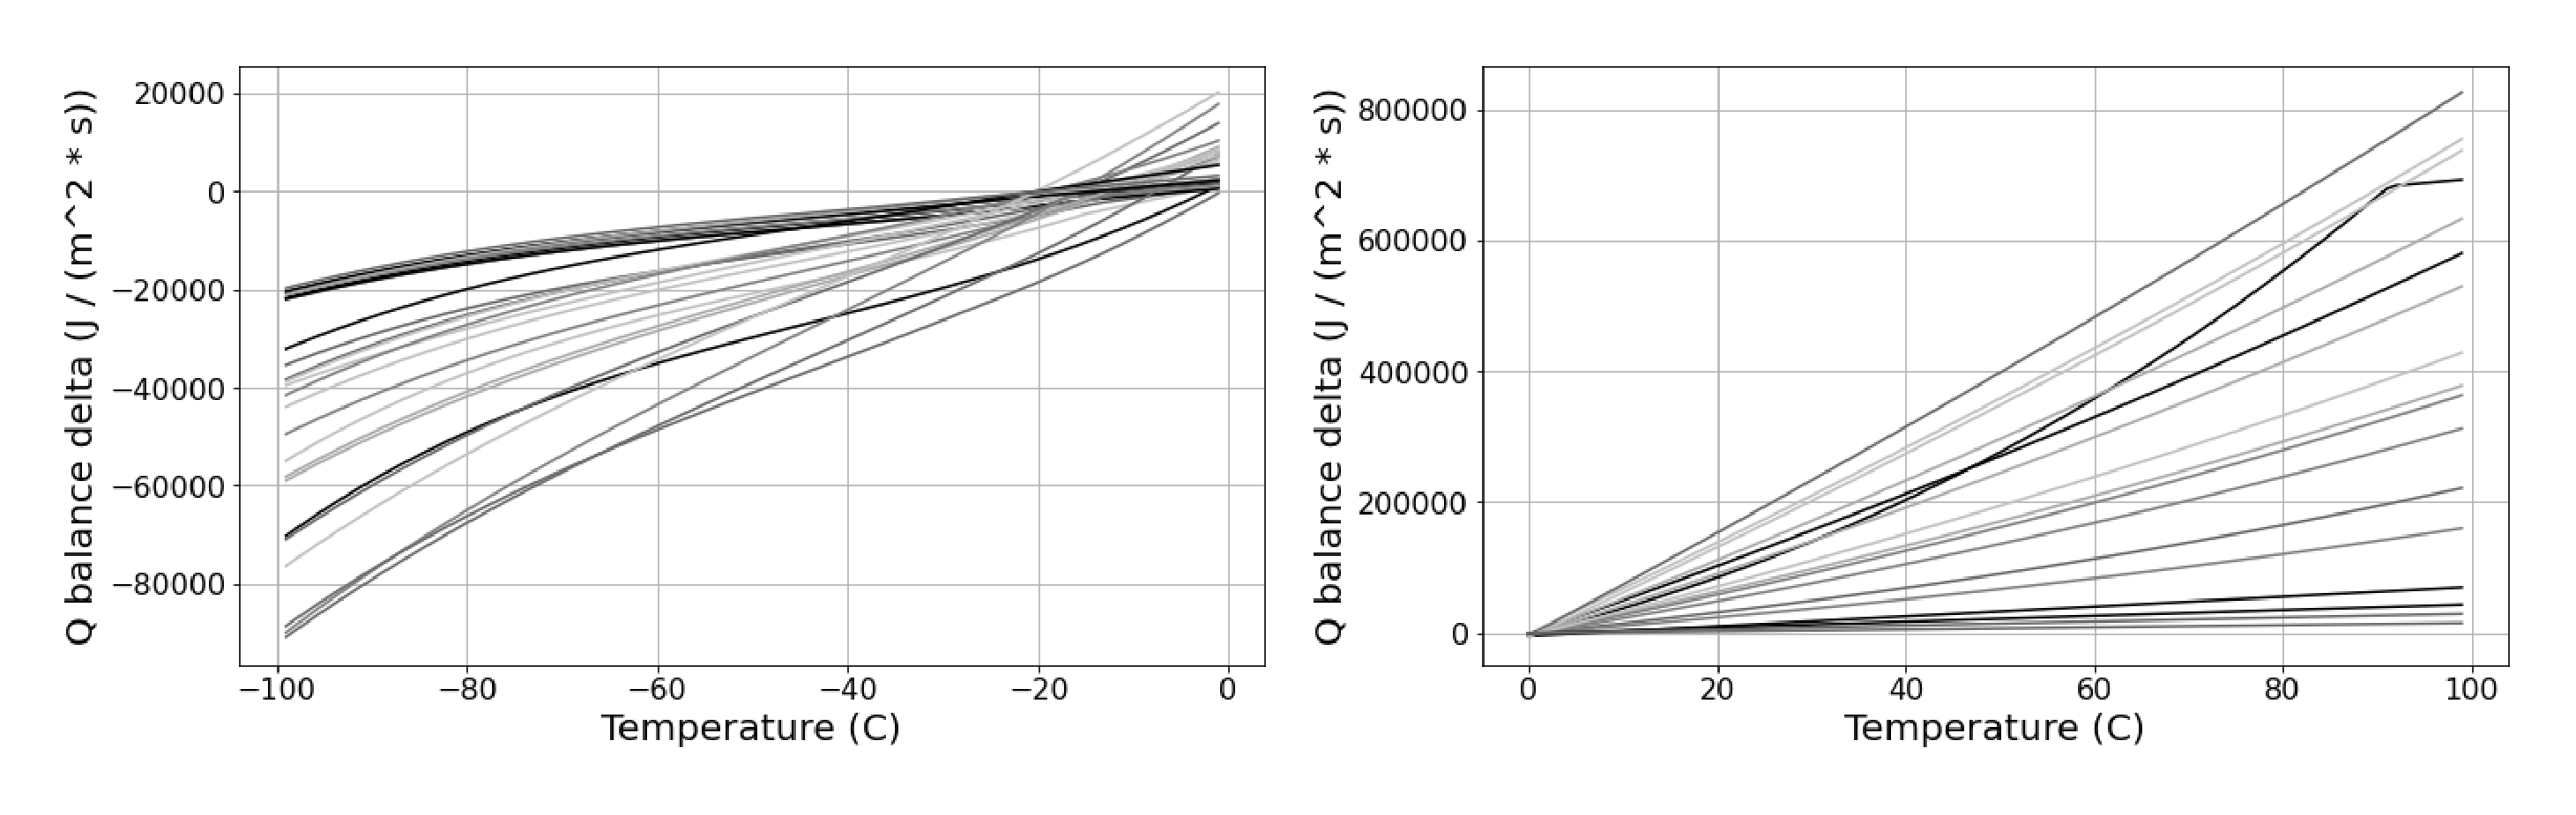
\includegraphics[width=1.0\textwidth]{pics/dq_rime_wet.pdf}
\captionstyle{normal}\caption{Семейсва графиков функций решения нелинейных уравнений при определения состояния ячеек rime ice (слева) и running wet (справа).}\label{fig:dq_rime_wet}
\end{figure}

\section{Methods of solving nonlinear equations}

Итак, мы рассматриваем решение нелинейного уравнения вида $f(x) = 0$, полученного из системы уравнений массового и теплового баланса для разрешения одного из состояний ячейки.
При выборе оптимального метода решения нелинейных уравнения для поставленной задачи использовались следующие методы: метод бисекций, метод хорд, метод Ньютона, метод Брента.
Уравнения решались в температурном интервале $x \in [-100, 200]$, для решаемых уравнений было выполнено условие $f(a) f(b) < 0$.

Метод бисекций рассматривался в качестве эталона для сравнения с другими методами, так как ясно, что он является наиболее медленным, зато гарантированно сходится при любых начальных условиях и любом виде анализируемой функции.
В процессе решения нелинейного уравнения методом бисекции интервал поиска на каждой итерации решения делится на два равные интервала, из которых выбирается один, для которого продолжает выполняться условие разнознаковости функции на концах интервала.

Метод хорд сход по смыслу с методом бисекций, однако на каждой итерации решения уравнения интервал поиска корня делится не на две равные части.
Точкой деления интервала поиска на два новых интервала определяется как пересечение оси $OX$ c отрезком $[(a, f(a)), (b, f(b))]$.
Данный метод в большинстве случаев приводит к более быстрому решению уравнения, однако возможны профили функций, для которых применение метода хорд может привести к катастрофическому замедлению процесса поиска корня.

На Fig.~\ref{fig:chords-newton} представлены схемы поиска корней нелинейного уравнения с помощью методов хорд и метода Ньютона.

\begin{figure}[h]
\setcaptionmargin{5mm}
\onelinecaptionstrue
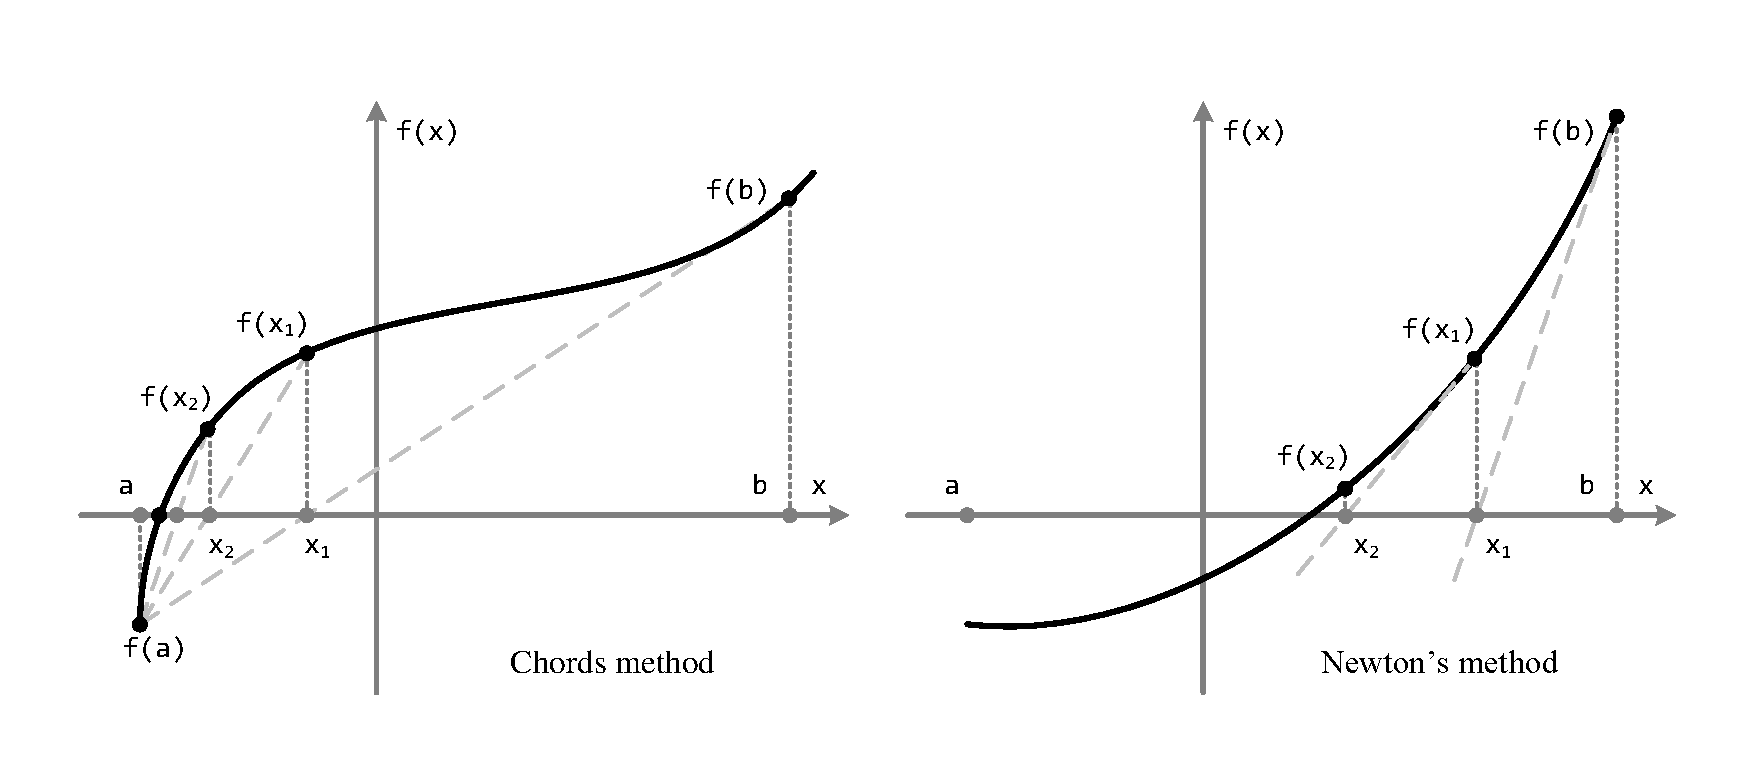
\includegraphics[width=1.0\textwidth]{pics/chords-newton.pdf}
\captionstyle{normal}\caption{Схемы поиска корня нелинейного уравнения методом хорд и методом Ньютона.}\label{fig:chords-newton}
\end{figure}

В методе Ньютона корень уравнения ищется начиная с некоторой точки (на Fig.~\ref{fig:chords-newton} начинаем с точки $b$).
Из данной точки проводится касательная до пересечения с осью $OX$ (что соответствует вычислению разностной производной с требуемым порядком точности) в некоторой точке $x_i$, которая и становится новым значением - кандидатом на корень уравнения.
Данный метод крайне эффективен для поиска корней уравнений, представленных, например, выпуклыми функциями, однако существуют профили функций, для которых метод Ньютона неприменим или может работать крайне медленно.

Метод Брента является модифицированным методом Деккера, который, в свою очередь, является объединением метода деления пополам с методом секущих.
В методе Деккера на каждой итерации происходит попытка применить метод хорд для сужения интервала поиска корня, а при невозможности применения метода хорд выполняется применение одной итерации метода бисекции.
В методе Брента осуществляется похожий синтез метода хорд и метода бисекций.
В этом методе также выполняется попытка применения метода хорд, а при снижении скорости стягивания интервала поиска корня применяются разовые итерации метода бисекций.
Кроме этого, линейная интерполяция в методе хорд заменена обратной квадратичной интерполяций.

\section{Numerical experiments}

Для анализа использования различных методов решения нелинейных уравнений были решены порядка 35000 уравнений, аналогичных уравнениям, показанным на Fig.~\ref{fig:dq}.
\newpage

\begin{table}[ht!]
\begin{tabular}{llll}
           & Failed, \% & Avg. func calls & Avg. iterations \\
bisections & 0.038      & 78.8            & 31.3            \\
chords     & 0.038      & 11.2            & 3.7             \\
newton     & 0.038      & 10.1            & 3.3             \\
brenth     & 0.038      & 5.5             & 4.5            
\end{tabular}
\end{table}

Принимая во внимание процент нерешенных уравнений, одинаковый для всех методов, можно сделать вывод, что эти уравнения не имеют решения на исследуемом интервале и это не связано с каким-либо методом. Распределение количества вызова функций и количества итераций представлено на Fig.~\ref{fig:calls} и Fig.~\ref{fig:iterations} соответственно. Анализируя распределения, видно, что наиболее эффективным в смысле количества итераций и количества вызовов функции является метод Брента.

\begin{figure}[h!]
\setcaptionmargin{5mm}
\onelinecaptionstrue
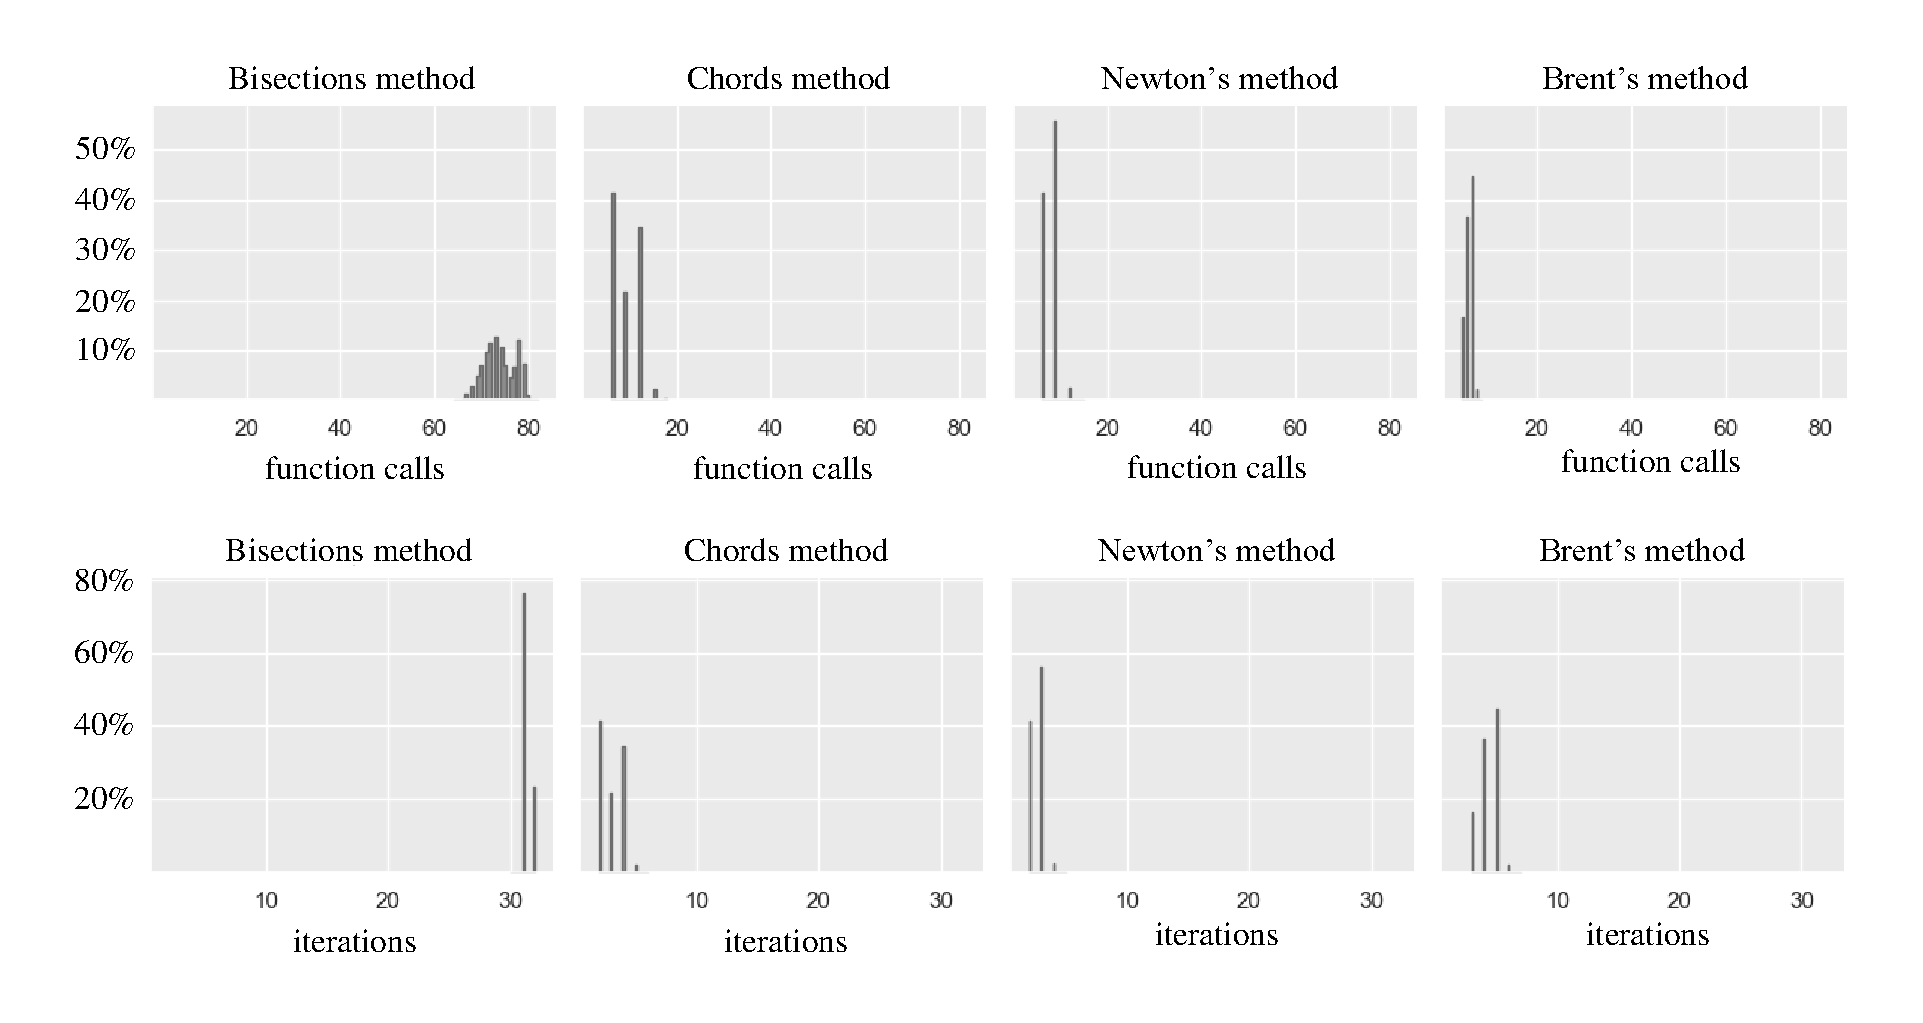
\includegraphics[width=1\textwidth]{pics/stat.pdf}
\captionstyle{normal}\caption{Статистика количеств вызово функции $f(x)$ и итераций решения нелинейного уравнения}\label{fig:stat}
\end{figure}

\section{Conclusion}

TODO

\begin{acknowledgments}
The work has been done at the JSCC RAS as part of the state assignment for the topic 0580-2021-0016.
The supercomputer MVS-10P OP, located at the JSCC RAS, was used during the research.
\end{acknowledgments}

\begin{thebibliography}{99}

\bibitem{Wright}
\refitem{article}
W.~W.~Wright, P.~Struck, T.~Bartkus, G.~Addy, {\it ``Recent Advances in the LIWICE Icing Model''}, SAE Technical Paper (2015).

\bibitem{Bourgault}
\refitem{article}
Y.~Bourgault, H. Beaugendre, W. G. Habashi, {\it ``Development of a Shallow-Water Icing Model in FENSAP-ICE''}, Journal of Aircraft, Vol. 37, No. 4, 640--646 (2000).

\bibitem{Beaugendre}
\refitem{misc}
H.~Beaugendre, {\it ``A PDE-Based Approach to In-Flight Ice Accretion''}, A thesis of the degree of Doctor of Philosophy, Department of Mechanical Engineering, McGill University, Montreal, Qu\'ebec (2003).

\bibitem{Dekker}
\refitem{article}
Brent, R.P.. Finding a zero by means of successive linear interpolation. : London, 1969.

\bibitem{Brent}
\refitem{book}
Brent, R.P.. Algorithms for minimization without derivatives. : Prentice-Hall, 1973.

\bibitem{Press}
\refitem{book}
William H. Press, Saul A. Teukolsky, William T. Vetterling, and Brian P. Flannery. 2007. Numerical Recipes 3rd Edition: The Art of Scientific Computing (3rd. ed.). Cambridge University Press, USA.


\end{thebibliography}

\end{document}
